\subsection{Problem Area}\label{sec:problemArea}
\comment{
Why are IoT Gateways so hard to get right? Why is the edge so hard to get right?
 - Diversity
 - Security
 - Stability
}
% Main text
{
Mobile devices profoundly changed the way computers interact with each other. When these devices became a commodity in the 90s\footnote{Back then smartphones were called personal digital assistant (PDA).}, the way we manage computing power needed to change to accommodate intensive tasks on light weight computers. Researchers started to experiment with local, remote (cloud) and mixed execution also called adaptive cloud offload. The researchers found huge gains from adaptive cloud offloading with a high enough bandwidth and concluded "the convergence of mobile computing and cloud computing enables new multimedia applications that are both resource-intensive and interaction-intensive."\cite{noble1997agileIoTGatewayOdyssey}. As one of the researches later put it "while mobile elements will undoubtedly improve in absolute ability, they will always be at a relative disadvantage."\cite{satyanarayanan2015briefHistoryIoTGateway}\\
In 2009, the National Science Foundation rejected a paper because \textit{``Many panelists do not agree with the premise of the proposal in which distant cloud computing incurs too high latency to be acceptable by mobile applications. They question the validity of such assumption as the proposal provides no real data to justify it[...]''}\cite{satyanarayanan2015briefHistoryIoTGateway}. Much has changed since then. The smartphone revolution greatly increased the data produced by mobile devices and the need for speed, security and privacy. Researches did not foresee the explosion in IoT and the onset of a new wave of data producers bundled under the term Indutrial IoT (IIoT). It includes hundreds and thousands of IoT devices working together in factories, logistic warehouses, connected vehicles (CV), smart grid etc. In 2012 a widely cited paper "Fog Computing and Its Role in the Internet of Things"\cite{fogComputing:def} was published, establishing the need for IoT gateways connected to the cloud. It concluded that the amount and high frequency of data produced in IIoT is too much for the cloud and core network to handle and pre-processing on the edge is needed for both latency and efficiency.\\
However, establishing the need for edge computing is not the same as solving it. Since then many papers have been published with titles such as "The Internet of Things Has a Gateway Problem"\cite{zachariah2015internetOfThingsHasGatewayProblem}. At the same time, researchers used custom IoT gateway solutions and achieved impressive results. In one experiment, they achieved over 80\% performance increase in certain scenarios rightly titling their paper "From Cloud Computing to Fog Computing: Unleash the Power of Edge and End Devices"\cite{hong2017fromCloudtoIoTGatewayUnleashingTHePower}.\\
This gateway problem stems from the fact that IoT devices are often build to last months on a single battery and have very limited processing power. New architectural patterns and communication technologies emerged to support these ultra low power and processing requirements which lead to a fractured landscape of IoT gateways where many manufacturers developed their own technology, mostly as closed source. There were some open source efforts but none taking over the entire industry. Applications running on these gateways were not isolated from the host operating system and often times security updates were not even deemed necessary. This left many IoT gateways and devices vulnerable to attacks. The Mirai botnet\cite{7971869MiraiAndOtherBotnetLinux} is a prime example where a maleware in 2016 brought down the Mirai domain name servers and caused an outage of several big websites. It is important to note, that most attacks target Linux devices and not microcontrollers. Thus, bringing the industry together on a standard for IoT gateways is in the best interest of everyone involved. 
}

\subsubsection{Expected Outcome}
This thesis will implement a fog system with Kubernetes at its core. It will explain how Kubernetes can aid in many challenges facing the edge and gives insights into important Kubernetes resources for the edge, including containers, and the best practices for using these resources. The developed system could become the industry norm influencing millions of deployments in many diverse industries. It would improve communication, observability and finally put a halt to most malicious attacks by greatly reducing the attack surface.\\

\subsubsection{Research Question}
In essence, the research question for this thesis is:
\begin{displayquote}\begin{center}
{\textit{\textbf{How can Kubernetes help facilitate edge and fog computing, what challenges does it solve and where are its shortcomings?}}}
\end{center}\end{displayquote}

\subsubsection{Delimitation} \label{sec:delimitation}
\comment{
Exclude non Kubernetes related technologies.\\
Exclude mobile devices.\\ All a lot of technologies are still relevant but not discussed. In future work mention it
Exclude hardware.\\
Exclude Sort of 5g and advances in mobile technologies.\\ Rich field
Exlude infrastructure edge.\\
Exclude RTOS.\\
}
This thesis is centered around Kubernetes and provides an exemplary implementation for edge/fog computing. Because Kubernetes and edge computing are both extensive topics this thesis will not discuss the following aspects in more detail:\\[5mm]



\textbf{\leftskip25mm\textit{Other Orchestration Technologies}}\\
Kubernetes is not the only container orchestration tool on the market, but its design and industry support has made the de-facto standard. Other tools like Apache Mesos\cite{ApacheMesos19:online} and Docker Swarm\cite{DockerSwarmmod12:online} are less adoptable than Kubernetes and not used as much. Rancher recently dropped support for both platforms in their new version saying that "out of more than 15,000 clusters, only about 200 or so are running Swarm"\cite{FAQ36RancherSwarmMesos:online}. I will follow this approach and only consider Kubernetes as orchestration platform.\\[5mm]
\textbf{\leftskip25mm\textit{Mobile Devices}}\\
Combing edge computing with mobile devices opens new doors for app developers and telephony companys (TelCos). This study concentrates on the IoT space with full awareness that many implications hold true for mobile devices as well. Because of their vast possibilities they deserve their own study.\\[5mm]
\textbf{\leftskip25mm\textit{Hardware}}\\
Advances in hardware play a huge role in enabling Kubernetes to run on edge devices, but it is not important for the technology itself. Kubernetes uses containers so even recent innovations in the hypervisor, especially on ARM, are not relevant.\\[5mm]
\textbf{\leftskip25mm\textit{5G}}\\
5G will enable even more devices to integrate with each other and connect to the Internet making edge computing even more important. Because of the low availability I will not consider the effects of 5G.\\[5mm]
\textbf{\leftskip25mm\textit{Real-Time Operating Systems}}\\
Real-time operating system (RTOS) can guarantee a certain time of execution and can be crucial for a specific business case. Linux can be patched to fulfill most real-time requirements and there are considerable efforts to bring Kubernetes and containers to fulfill real-time requirements. It is especially important paired with 5G and emerging technologies like autonomous cars\cite{CNCFLaunRTOSKubernetesContainers40:online}. All this is outside the scope of this thesis but very interesting and could open up even more use cases for Kubernetes.\\[5mm]
\textbf{\leftskip25mm\textit{Cloud Computing Models}}\\
How the hard and software is provided to the customers and its effects are also outside of this thesis scope and the concepts are only shortly explained here. A customer can purchase online computing space and run Kubernetes herself. This is called Infrastructure as a Service (IaaS). It is also possible to get a managed version of Kubernetes so called Platform as a Service (PaaS). Finally, Software as a Service (SaaS) is were the customer only pays for the final software. 






\comment{


Edge computing started as a way to give mobile devices more power.
Technopedia defines a mobile device as a "handheld tablet or other device that is made for portability, and is therefore both compact and lightweight"\cite{WhatisaM95TechnopediaMobileDevice:online}, it includes laptops, smartphones, tables etc.  As Mahadev Satyanarayanan put it "while mobile elements will undoubtedly improve in absolute ability, they will always be at a relative disadvantage."\cite{satyanarayanan2015briefHistoryIoTGateway} Back then, researchers experimented with local, remote (cloud) and mixed execution also called adaptive
cloud offload. Assessing the three variants for voice recognition, video playback and web browsing locally, the researchers found huge gains from adaptive cloud offloading with a high enough bandwidth and concluded "the convergence of mobile computing and cloud computing enables new multimedia applications that are both resource-intensive and interaction-intensive."\cite{noble1997agileIoTGatewayOdyssey}. This lead to an explosion in cloud development. The Internet started out with a decentralized servers around the world. But over the years technologies were invented for orchestration across these distant servers, but also isolation for the local deployments. Probably the two main technological standards evolving where containers with containerd and orchestration with Kubernetes. \\
Traditionally, mobile devices connected to a gateway, which was mainly a router operating at L3\footnote{L3 stands for Layer 3, the networking layer in the OSI model.} to route packets and translate between different types of network protocols. \cite{lee2017futureOfIoT}. However, according to Dejan Bosanac, a senior software engineer at Red Hat in the field of cloud messaging and IoT platforms, due to their proximity to the sensors and the end user, these devices have three main advantages over the cloud: 
\begin{displayquote}
{\textbf{``Low latency, availability and locality''}}\cite{IntroducingDejanBosanac:KubernetesIoTEdgeWorkingGroup} - Dejan Bosanac.
\end{displayquote}
Because of these advantage researchers construct hybrid systems, in which devices operating on the edge of the network play an active role in the data processing pipeline. This architectural style of carrying out substantial amount of computation and storage at the edge is called "edge computing" \cite{fogComputing:def}. \Cref{fig:iotDeviceSetup} shows where the gateway is positioned in the current communication setup. 
 \begin{figure}[!h]
     \centering
     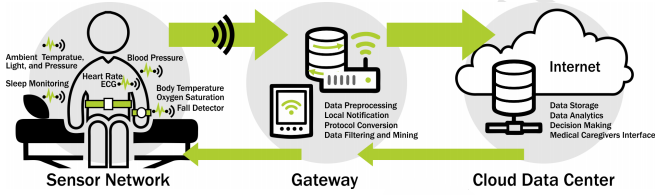
\includegraphics[scale=2]{figures/iotSetup.png}
     \caption{The position of the gateway in the current Internet infrastructure\cite{iotGatewaySlavesGraph}.}
     \label{fig:iotDeviceSetup}
 \end{figure}\\
But not everyone in the academic world was convinced that edge computing was indeed the way forward. 
However, establishing the need for edge computing is not the same as solving all problems though, and since then many papers have been published with titles such as "The Internet of Things Has a Gateway Problem"\cite{zachariah2015internetOfThingsHasGatewayProblem}. At the same time, researchers used custom IoT gateway solutions in their research and achieved impressive results. In one experiment, they achieved over 80\% performance increase in certain scenarios rightly titling their paper "From Cloud Computing to Fog Computing: Unleash the Power of Edge and End Devices"\cite{hong2017fromCloudtoIoTGatewayUnleashingTHePower}. Adding further to the problem of standardization is that IoT, especially IIoT, and mobile device have very different requirements.\\
This is the current place of the industry. There is a common agreement that fog computing is essential in the future, but no standard and open solution was developed yet. There is considerable effort in the academic world and in the industry to establish such a standard, one such initiatives is the Kubernetes IoT Edge working group under the Cloud Native Computing Foundry (CNCF). 




The space between the cloud and IoT and mobile devices, can be confusing at times. Knowing the history of IoT and the cloud is vital to understand the current developments. This, the methodology and the delimitation of this thesis will be discussed in the reminder of this section.\\




The terms used in the academic world and the industry are often different and many concepts partially overlap and complement each other making it hard to clearly categorize solutions. This is mainly due to ever evolving hard- and software, changing the possibilities of the devices and the entire landscape. It is thus imperative to clearly outline the key terms and design philosophies used of this thesis as well as presenting already existing solutions and how they compare to each other. These aspects are part of \cref{sec:eSOTA}, \nameref{sec:eSOTA}.\\
\Cref{sec:analysis}, \nameref{sec:analysis}, will lay the foundation to the actual implementation. We will motivate our design choices with academic and industry literature as well as with interviews from industry leaders. The focus of this thesis will be on the software and the requirements of the software to define and use the edge. Ultimately, it does not matter whether increases in performance and security come from better hardware or software, as long as the requirements are met. Consequently, the requirements will be ordered via the MoSCoW method. I will analyze the existing protocols, mainly for the application layer, and the data serialization method. Kubernetes is at the heart of this thesis implementation and extra sections will discuss what tricks Kubernetes already offers to control an edge cluster from the cloud and what might be missing. Additionally, I will look at extensions Kubernetes offers and how they could be useful in an IoT environemnt.\\


}

\comment{
The main focus is going to be on the software driving fog computing with an emphasize on IoT device and less mobile devices. 
We use a three tier layered network topology shown in \cref{fig:networkTopology3Layer}.
\begin{figure}[h!]
    \centering
    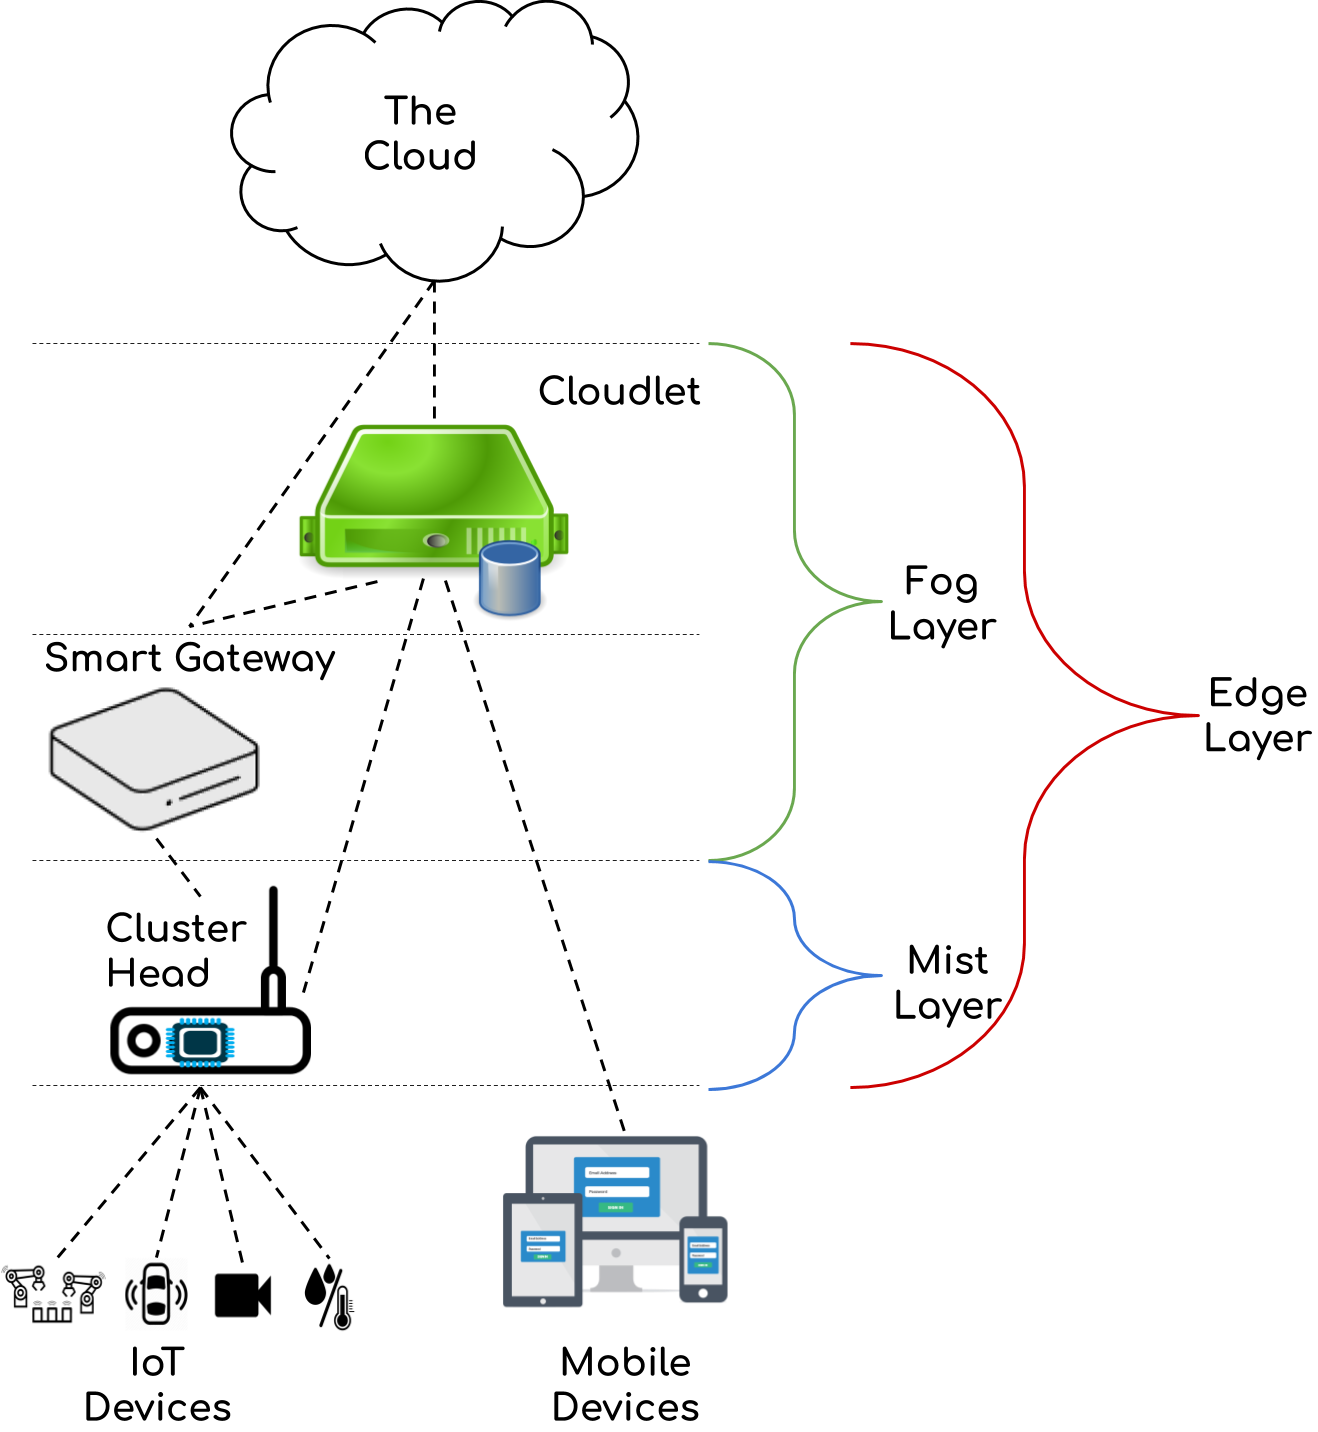
\includegraphics[scale=0.15]{figures/network-topology-3-layer.png}
    \caption{Three tier layer network topology, similar to \cite{nsa2017theNextWaveIoTDefinitions}}
    \label{fig:networkTopology3Layer}
\end{figure}
% Describe figure:
The cloud layer is made up of the 

% More detail
The cloud is the one layer where the authors think the technology stack is set. We expect Linux and Kubernetes, the de-facto standard for cloud orchestration, to be here to stay for the foreseeable future. This implies the same for x86\_64 and ARM, the only CPU architectures being supported by Linux. The Internets communication will remain in IPv4 and increasingly IPv6 for the Internet layer and TCP and UDP for the transport layer.\\ 
Quite the contrary is true for the bottom layer, IoT devices and mobile devices, although for the latter to a lesser extend. Communication in the IoT space is very diverse. Some protocols like 802.11 and Mobile

We expect IoT devices to have different software and different 
This can, but must not, include a control plane
The aim is to find the most promesing solution and 




Promesing solution with deep integration into K8s.


In essence, fog is the standard, and edge is the concept. Fog enables repeatable structure in the edge computing concept, so enterprises can push compute out of centralized systems or clouds for better and more scalable performance.
https://www.cisco.com/c/en/us/solutions/enterprise-networks/edge-computing.html


As it's name implies its aim is to develop an edge solution with Kubernetes support.

The need for smart IoT Gateways or fog computing is well established. They make it possible to 

Their design however is not. 
While the problems at the IoT edge — connectivity, manageability, scalability, reliability, security — are being solved as point solutions by enterprises and ecosystem players, there is a need for a foundational industry-wide standard for managing distributed IoT workloads.





IoT has seen a rapid growth over the last few years. According to IoT Analytics the total number of IoT devices is set to surpass the total number of other connected devices around 2021 \cite{StateofIoT:online}. Further, most IoT devices will be used in WPAN \footnote{Wireless Private Area Networks includes technologies like Zigbee,Z-wave and Bluteooth} and WLAN\footnote{Wireless Local Area Networks includes mainly Wi-Fi}. 
% In contrast to 5G, these technologies don't connect to an access point from an Internet provider but rather require another user operated device to connect to the Internet, a so called "gateway"


But fog computing does not come without its drawbacks. Depending on the protocol edge devices need to be close to their peers and slaves and physically accessible for maintenance. Which also poses a major security risk as they could be accessed by malicious intruders. The software maintenance is another critical aspects. Often IoT and edge devices are not update and patched with critical consequences. The "2016 Dyn cyberattack" used IoT devices like residential gateways, smart fridges, baby phones ect. to bring down the DNS-Servers operated by Dyn making large part of the Internet unaccessible for hours\cite{dynAttack}. The authors also stress that "large number of IoT devices are accessible over public Internet" and that "security (if considered at all) is often an afterthought in the architecture of many wide spread IoT devices"\cite{dynAttack}.\\
The question is then, how can manage and secure those devices. In this thesis, I will solely be concerned with the software aspect, which can mitigate some effects of exposing physical hardware to more accessible places.\\
Many challenges facing edge devices today have already been solved, although in a slight different context: The cloud\cite{IntroducingDejanBosanac:KubernetesIoTEdgeWorkingGroup}. In the cloud 




% Note: Maybe make a graph cloud setup, user connecting to nodes, VS fog computing, sensors and users connecting to gateways and gateway to cloud.  https://www.einfochips.com/blog/iot-gateways-drivers-for-fog-computing/

Kubernetes IoT Edge Working Group is a collaboration between Eclipse IoT Working Group and its 40-member companies, 35 open source projects, and Kubernetes ecosystem. It will define terminology, identify gaps in deployment and management, and educate the market on common use cases.
https://www.dailyhostnews.com/eclipse-foundation-and-cncf-working-together-to-bring-kubernetes-to-iot-edge
}